\graphicspath{{content/1_literatureReview/figures/}}
\section{PWM to Analog Conversion}\label{sec:pwmAnalogConversion}

PWM (Pulse Width Modulation) is useful in that it allows analog information to be conveyed in digital signals.
PWM waves are similar to square waves, however differ in that $t_{high} \neq t_{low}$. A PWM signal is defined by 3 properties:
\begin{itemize}
    \item Frequency: The rate at which the signal oscillates. $f = \frac{1}{t_{high} + t_{low}}$ Hz.
    \item Amplitude: The difference between "high" and "low" voltages. $A = V_{high} - V_{low}$ V.
    \item Duty cycle: The ratio of the signal's "high time" to its period. $\tau = \frac{t_{high}}{t_{high} + t_{low}}$ s.
\end{itemize}

\begin{figure}[!htb]
  \centering
  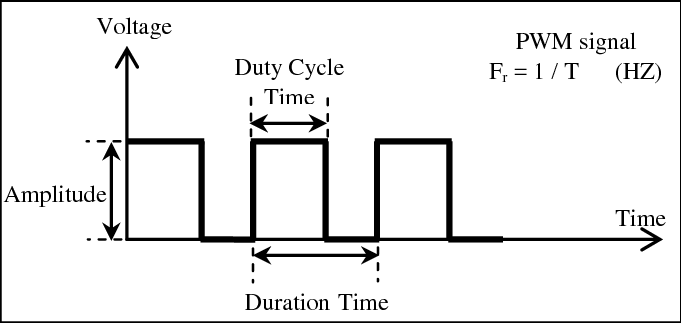
\includegraphics[width=0.25\textwidth]{pwm_graph}
  \caption{PWM Signal Voltage vs Time \cite{pwmGraph}}
\end{figure}

Often, this analog information is conveyed in a varying duty cycle ($\tau$). To convert this varying value to analog,
a low-pass filter can be used. Since the signal's average value increases with $\tau$, filtering out all "harmonics" of the
signal will result in \inlineequation[eqn:pwm_filtered_amplitude]{V_{out} = A \times \tau} \cite{pwmAnalogConversion}. The cutoff frequency ($f_{c}$) of the filter
should be as low as possible, while maintaining an acceptable rise time, in order to minimize ripple on the filter output.
Then, since $t_r \propto \frac{1}{f_c}$, $t_{r(max)}$ will determine the minimum cutoff frequency, $f_{c(min)}$. This will be based on the filter used
e.g. $f_{c(min)}$ = $\frac{3.3}{2 \pi \cdot t_{r(max)}}$ for a \nth{2} order filter [\ref{filter_formulae}].

\begin{figure}[!htb]
  \centering
  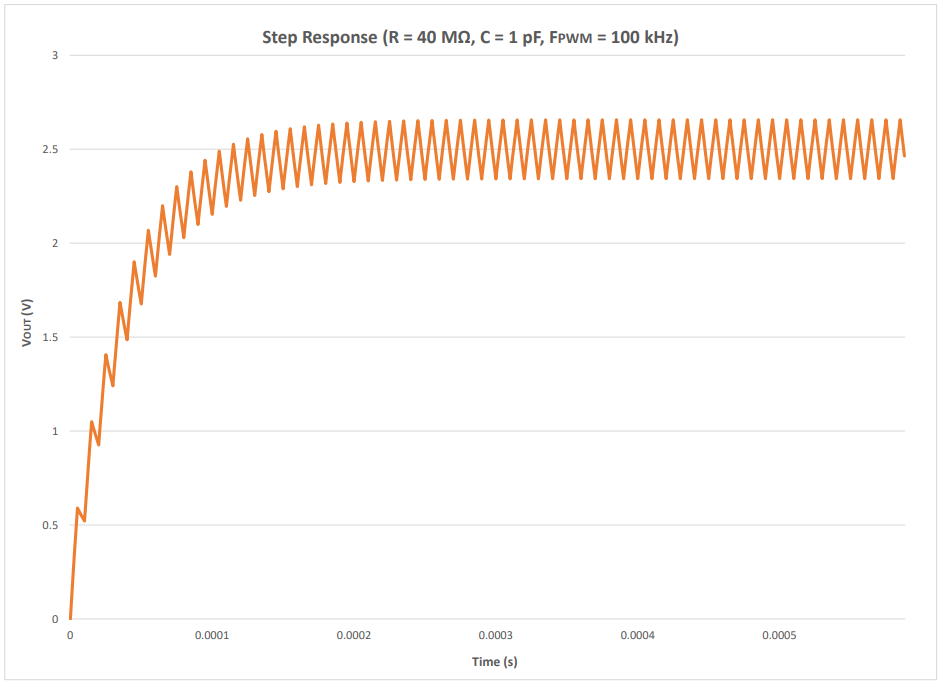
\includegraphics[width=0.3\textwidth]{pwm_filtered}
  \caption{Filtered PWM signal}
\end{figure}

Assuming $f_{c(min)}$ is fixed, $f_{c(max)}$ should be determined by the maximum acceptable noise on the output of the filter.
Since filtering will still leave a small "ripple" signal at frequency $f_{PWM}$, this will be the largest noise component. Given the following:
\begin{itemize}
  \item $A$: Amplitude of the PWM signal (V)
  \item $\tau_{max}$: Maximum duty cycle of the PWM signal (\%)
  \item $N_{max}$: Maximum acceptable noise of the filtered output (V)
\end{itemize}

\noindent Then the required attenuation at $f_{PWM}$ is given by \inlineequation[eqn:pwm_required_attenuation]{A_{dB} = 20 \log \left[ \frac{A \cdot \tau_{max}}{N_{max}} \right]}.
This will determine $f_{c(max)}$, in conjunction with the type of filter used and its order.